%!TEX root = ../thesis.tex

\chapter{Experiment}
\label{ch:eval}

\section{Usecases and Overview}
We take inspiration from a supply chain network to design the workflow that will allow organizations to share datasets and other organizations to consume them without exposing the data itself. We think of data as an asset comparable to a physical asset, and use a blockchain as a centralized ledger between organizations to lease the data back and forth. The use of blockchain ledger allows the organizations to maintain their ownership over their datasets without trusting a third party maintaining the system, while others could lease and use the data to perform some analytics.

\bigskip
To test the system we design two main experiments to demonstrate the two different sources where data could be stored to be consumed by this proof of concept and also to demonstrate linear and parallel workflow design. In the next section, we will demonstrate how we can deploy the system and set it up for testing. Most of the same procedure can be used to set it up on VMs to set up a production environment. And finally, we will discuss the following two scenarios and how their workflow files are constructed and data sources for tests:

\begin{itemize}
    \item The workflow is linear and the data is hosted on a Kubernetes node.
    \item The workflow is parallel and results are combined and also the data for these parallel jobs are sourced in Azure File Shares.
\end{itemize}

\section{Deploy the System and Setup}
As \ref{fig:overview} highlights we have a couple of components that need to intercommunicate. So we will divide this deployment into two sections. In section one we discuss the deployment of the Hyperledger Fabric network and the REST API on a machine. And in the next section, we discuss building and deploying a JupyterHub server on a Kubernetes cluster. 

\subsection{Deploy Hyperledger Fabric}
In a production-ready system, each organization will set up Hyperledger on their own machines or nodes and join them to a network. We have already discussed the steps to join peers in a network. For the test here we use Docker to spin up nodes belonging to different organizations. We spin up a network with two participating organizations and a third orderer organization. And as the next step, we add a third participant organization or the fourth organization in total to this network. The docker-compose setup also starts certified authorities for the organizations.

\bigskip
It is recommended to run this on a machine separate from the Kubernetes cluster and accessible on a public IP since the project is configured to call a hard-coded IP from the browser and a Kubernetes headless service with the same IP. The pre requisites for the setup are Docker, Docker Compose, NodeJS, and NPM for the REST API. Following are the outlined steps to spin up and start a Hyperledger Fabric network with the chaincode and a REST API with Redis Cache and MySQL database on a machine using docker.

\begin{enumerate}
    \item SSH into the machine and get a shell session into the machine.
    
    \item Clone the repository for this thesis. \url{https://github.com/aliakbarrehman/master-thesis-uis}
    \begin{lstlisting}[language=bash]
    git clone https://github.com/aliakbarrehman/jupyterflow && cd master-thesis-uis\end{lstlisting}
    
    \item Run the following commands. The Script installs the Pre-Requisites as well as spins up the network with keys in \lstinline{hyperledger-network/crypto-config}, installs the chaincode for all organizations and spins up Rest API as well as Redis Cache and MySQL database.
    \begin{lstlisting}[language=bash]
    chmod +x spinUpNetwork.sh
    sudo ./spinUpNetwork.sh\end{lstlisting} 
\end{enumerate}

After the script finishes running the containers for certificates authorities, peers and chaincode containers for all organizations and orderer organizations along with the API, Redis and MySQL containers should be up. If the script run successfully \lstinline{docker ps} should show the output as in \ref{fig:vm-containers}

\begin{figure}
    \centering
    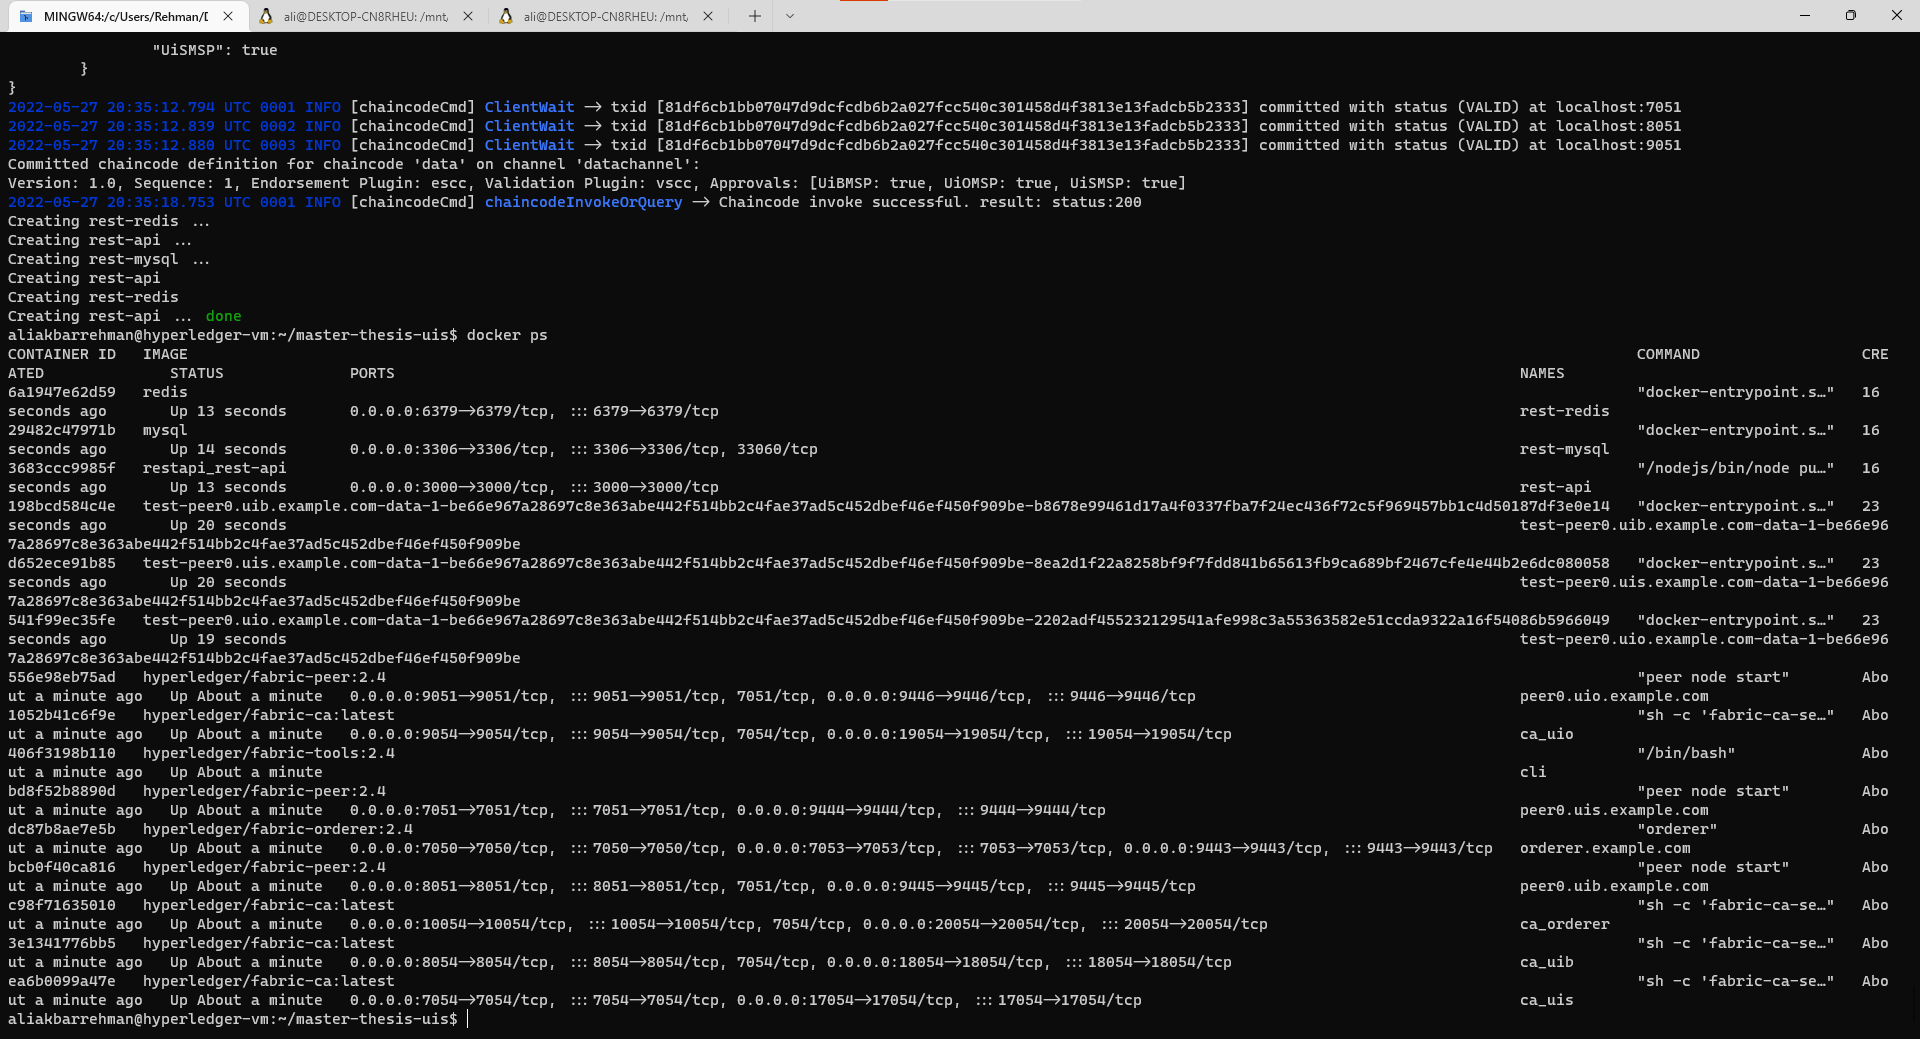
\includegraphics[width=14cm,keepaspectratio]{photos/Hyperledger-vm.png}
    \caption{The containers running on the Hyperledger VM after running the \lstinline{spinUpNetwork.sh} script successfully}
    \label{fig:vm-containers}
\end{figure}

\subsection{Deploy JupyterHub on Kubernetes}
The next component to set up for the demo is JupyterHub on Kubernetes. The pre requisites are Docker, NodeJS, NPM, Python, PIP, Kubernetes, and helm. The pre-requisites need to be installed following their respective setup instructions. Refer to the links in the footnotes for individual instructions.
\footnote{\url{https://docs.docker.com/engine/install/ubuntu/}}
\footnote{\url{https://github.com/nodesource/distributions/blob/master/README.md}}
\footnote{\url{https://linuxize.com/post/how-to-install-pip-on-ubuntu-20.04/}}
\footnote{\url{https://microk8s.io/\#install-microk8s}}

\begin{enumerate}
    \item Clone the repository for this thesis. \url{https://github.com/aliakbarrehman/master-thesis-uis}
    \begin{lstlisting}[language=bash]
    git clone https://github.com/aliakbarrehman/jupyterflow && cd master-thesis-uis\end{lstlisting}
    
    \item Change IP in \lstinline{jupyterhub/extension/thesis_extension/src/utils/api.ts} and
    \lstinline{jupyterhub/blockchain-service.yaml} with the public IP of the Hyperledger network as obtained from the previous section setup.
    
    \item Create a docker registry account and login to it \lstinline{docker login hub.docker.com}
    
    \item The first step to set up JupyterHub on Kubernetes is to build the extension and JupyterFlow into pip packages and build a docker image that will be used to spin up Jupyter Server for each user that logs in. We can run the \lstinline{buildJupyterhub.sh} with your docker hub repository.
    \begin{lstlisting}[language=bash]
    chmod +x jupyterhub/*.sh
    ./buildJupyterhub.sh aliakbarrehman/jupyterhub\end{lstlisting} 
    
    \begin{itemize}
        \item This script first creates a Kubernetes service account with permissions to manage secrets, persistent volumes, and persistent volume claims.
        \item Next it packages extension from \lstinline{jupyterhub/extension/thesis_extension}, extracts the wheel package name and copies it into docker context.
        \item Next the script packages our developed JupyterFlow from \lstinline{jupyterhub/jupyterflow}, extracts the wheel package name, and copies it into docker context.
        \item And finally the script builds a docker image with the extension and JupyterFlow installed and configured and the service account token set in environment variables. 
    \end{itemize} 
    
    \item Change \lstinline{singleuser.image.name} and \lstinline{singleuser.image.tag} in \lstinline{jupyterhub/config.yaml} with your own.
    
    \item Run \lstinline{./runJupyterhub.sh}. This script installs the JupyterHub from the helm charts, and the Argo workflow from helm charts, creates the load balancing services and creates roles, and binds them to the Argo workflow.
\end{enumerate}

\bigskip
Finally, once both the systems have been deployed, JupyterHub should be accessible on port 80 (\url{http://localhost}) and the Argo Workflow dashboard should be accessible at port 2746 (\url{https://localhost:2746}). And now users can log in to the JupyterHub and use the extensions to explore datasets, write code to consume datasets and trigger workflows that can be monitored on the Argo dashboard.

\section{Experiments}
\subsection{Linear Workflow with Local Dataset}
In the first experiment, we create two blocks on the blockchain for local datasets. By local here we mean datasets on the Kubernetes node. The workflow is linear where each job is run after the previous job has succeeded. The workflow for this example is presented in the listing \ref{lst:simple-wflow} The Ids are received when the user clicks to use a data.

\begin{lstlisting}[language=python,caption={Simple linear workflow.yaml consuming data from the Kubernetes node},label={lst:simple-wflow}]
jobs:
- command: 'ls /home/jovyan/'
- command: 'ls /home/jovyan/uis > result.txt'
  volumes:
  - id: '6de22e830ce4661cbeb6b9b2167c3f206dd946eb89beecd2f20bb17e85e64995'
    name: 'uis'
    path: '/home/jovyan/uis'
- command: 'ls /home/jovyan/uio >> result.txt'
  volumes:
  - id: 'e8a019a72cd8da522f620ab5561f5ada0143ea136ef71d8e601f6007c9386269'
    name: 'uio'
    path: '/home/jovyan/uio'

# Job index starts at 1.
dags:
- 1 >> 2
- 2 >> 3
\end{lstlisting}

When JupyterFlow is triggered with the command \lstinline{jupyterflow run -f workflow.yaml}, it mounts the data at \lstinline{/home/jovyan/uis} and \lstinline{/home/jovyan/uio} respectively. As dags (Directed Acyclic Graphs section) of the workflow state, the workflow is linear. It generates the Argo workflow as shown in \ref{fig:linear-wflow}

\begin{figure}
    \centering
    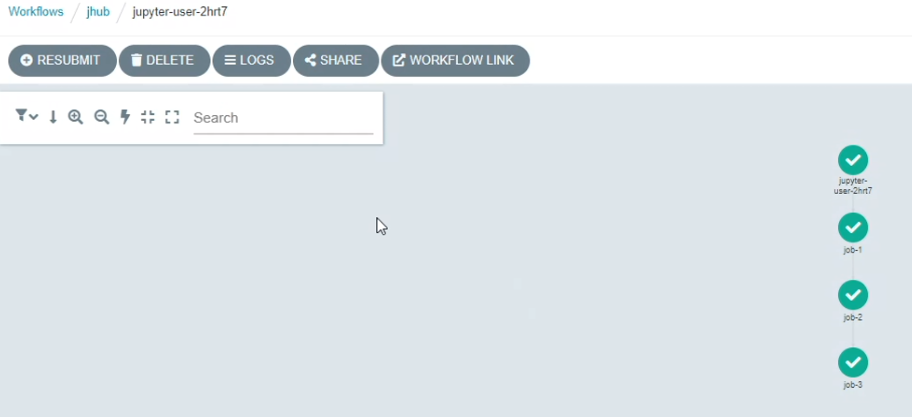
\includegraphics[width=10cm,keepaspectratio]{photos/linear-wflow.png}
    \caption{Linear workflow generated by the YAML file shown in listing \ref{lst:simple-wflow}}
    \label{fig:linear-wflow}
\end{figure}

\subsection{Complex Workflow with Azure and Local Datasets}

\begin{figure}
    \centering
    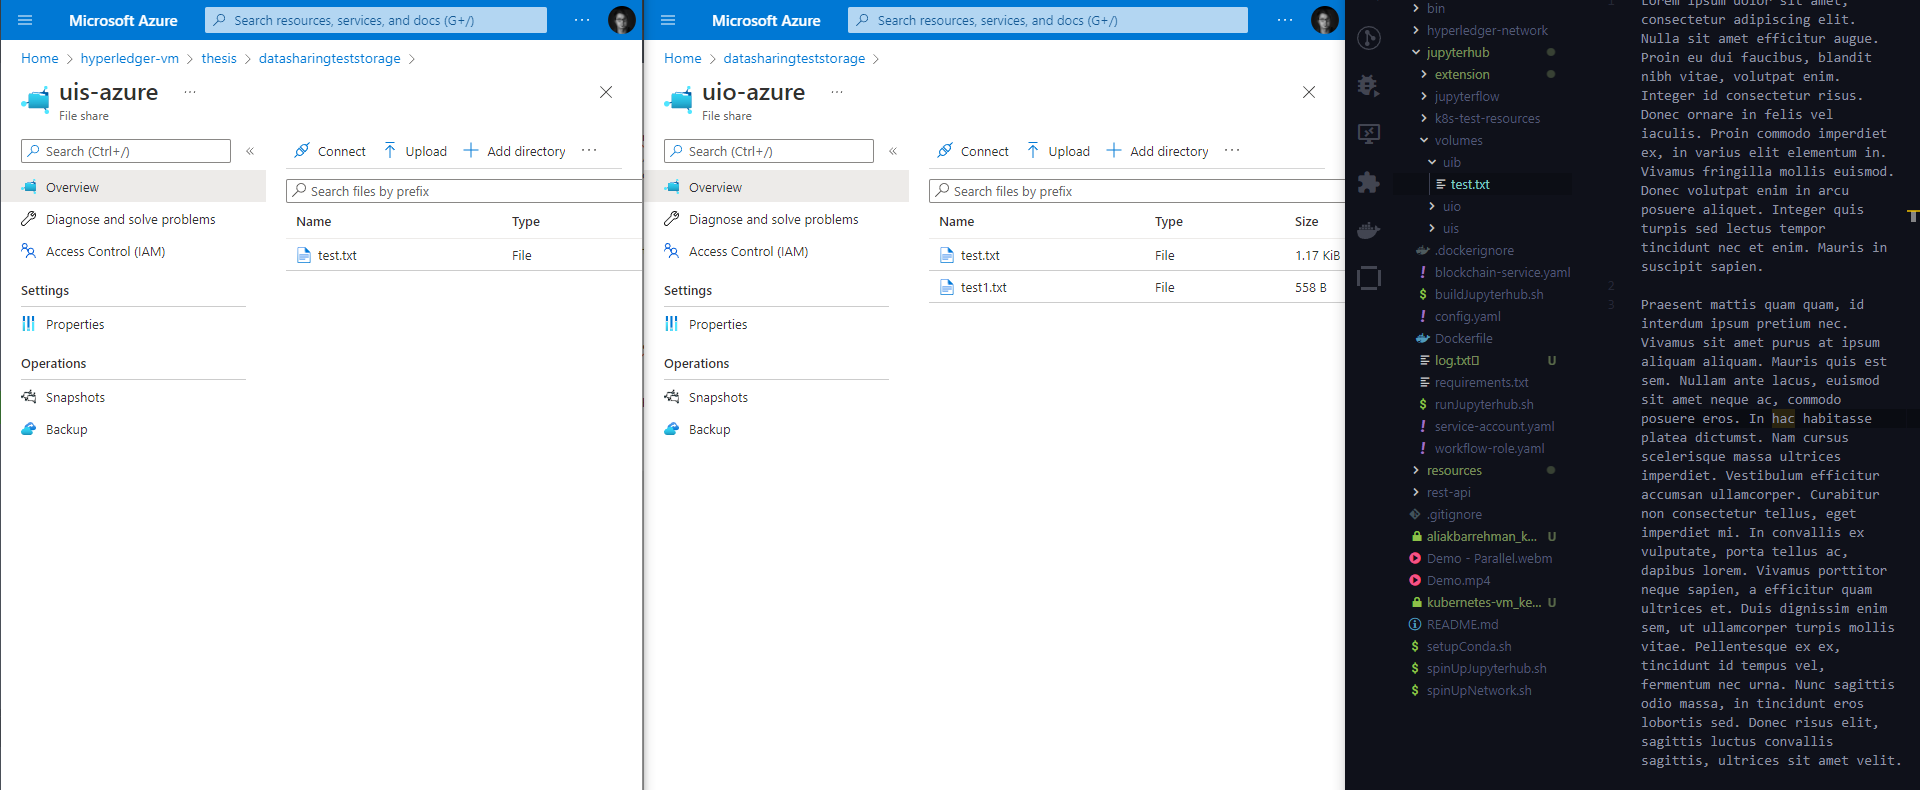
\includegraphics[width=14cm,keepaspectratio]{photos/dataset.png}
    \caption{Datasets for the complex workflow example. Azure File Shares and local dataset shown in VSCode}
    \label{fig:datasets}
\end{figure}

In the second experiment, we design and run a complex workflow that runs jobs in parallel and combines the results from them in the last job. Moreover, each job consumes data from different data sources. Two datasets are hosted in an Azure Storage Account in two different File Shares and the dataset for one job is hosted on the Kubernetes node itself.

\bigskip
In this experiment, we have the data hosted in azure and locally on the Kubernetes node as shown in the \ref{fig:datasets} datasets for UiO and UiS are in Azure and UiB hosted their data on the Kubernetes node. UiO, UiS, and UiB are test organizations and we have no formal dataset agreement for this demo.

\bigskip
The listing \ref{lst:parallel-wflow} shows the workflow.yaml for this experiment that JupyterFlow consumes. Dags section here sets up the workflow to run parallel jobs. And the last job combines and outputs the result of the workflow. The Ids are received when the user clicks to use data. This produces the \ref{fig:parallel-wflow} workflow in Argo.

\begin{lstlisting}[caption={Complex workflow consuming data from Azure},label={lst:parallel-wflow}]
jobs:
- command: 'ls /home/jovyan/'
- command: 'python uis.py'
  volumes:
  - id: '36b0c4d057e1bf9c0915e66330d18299d0f08c0c0f0340847cc879b3fbf73b4d'
    name: 'uis'
    path: '/home/jovyan/uis'
- command: 'python uio.py'
  volumes:
  - id: 'c12e28fb1d8c4bb243d5e7622afd90fde92ddb53971be384b92c33a464c80451'
    name: 'uio'
    path: '/home/jovyan/uio'
- command: 'python uib.py'
  volumes:
  - id: '3011ffd02613bb0971fb14b3bcbfea54ab1141afcd78c06ca18337f29740abbc'
    name: 'uib'
    path: '/home/jovyan/uib'
- command: 'python final-result.py'

dags:
- 1 >> 2
- 1 >> 3
- 1 >> 4
- 2 >> 5
- 3 >> 5
- 4 >> 5
\end{lstlisting}

\begin{figure}
    \centering
    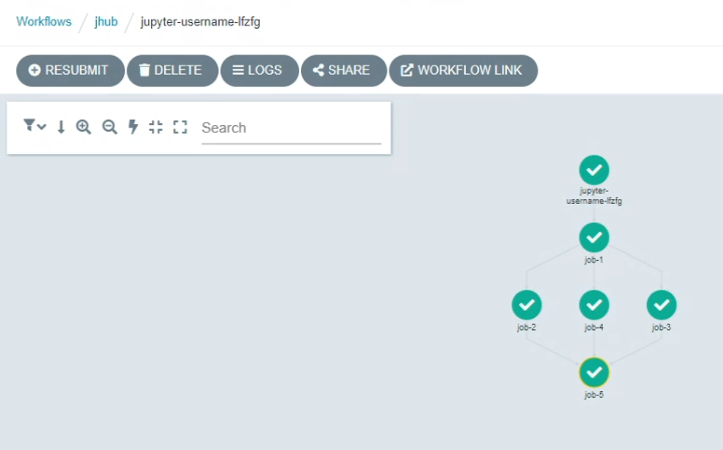
\includegraphics[width=10cm,keepaspectratio]{photos/parallel-wflow.png}
    \caption{Parallel Workflow generated by the YAML file shown in listing \ref{lst:parallel-wflow}}
    \label{fig:parallel-wflow}
\end{figure}

\bigskip
The listings \ref{lst:uis-py} and \ref{lst:final-result-py} show the python code that is run for each job in the complex workflow. The code counts the occurrences of work \textbf{lorem} in files under a dataset. And the \lstinline{final-result.py} has code that aggregates and outputs the final results to a file.

\begin{lstlisting}[language=python,caption={uis.py similar to uio.py and uib.py. The code that is run for the parallel jobs},label={lst:uis-py}]
import os

path = '/home/jovyan/uis'
files = []
for (dirpath, dirnames, filenames) in os.walk(path):
    for i in filenames:
        files.append(os.path.join(dirpath, i))
    break
    
count = 0
for i in files:
    f = open(i, 'r')
    for line in f:
        count += line.count('lorem')

f = open('/home/jovyan/uis-count.txt', 'a')
f.write('UiS: ' + str(count) + '\n')
f.close()
\end{lstlisting}

\bigskip

\begin{lstlisting}[language=python,caption={final-result.py that combines the output of the parallel jobs and computes the output},label={lst:final-result-py}]
import os

path = '/home/jovyan/uis'
files = ['uis-count.txt', 'uio-count.txt', 'uib-count.txt']

result = ''
for i in files:
    f = open(i, 'r')
    for line in f:
        result += line + '\n'

f = open('/home/jovyan/result.txt', 'a')
f.write(result)
f.close()
\end{lstlisting}

A complete demonstration of the experiments can be found at \url{https://github.com/aliakbarrehman/master-thesis-uis/blob/master/Demo\%20-\%20Parallel.webm} and \url{https://github.com/aliakbarrehman/master-thesis-uis/blob/master/Demo.mp4}